\subsection{Overview}
This section introduces modules and workflow of this tool.

\begin{figure}[htp]
    \centering
    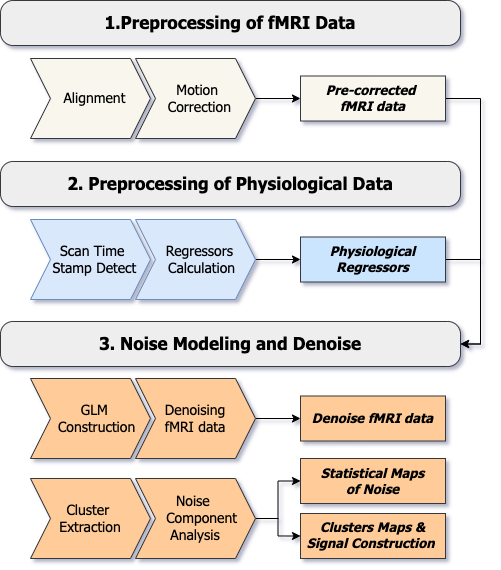
\includegraphics[width=\columnwidth]{Figures/modules.png}
    \caption{Workflow of Denoise Tool}
    \label{fig:modules}
\end{figure} 

This tool consists of three main modules, as depicted in Fig.\ref{fig:modules}, 
including preprocessing of fMRI data, preprocessing of physiological data  and noise modeling.
Briefly, the first modeule preprocesses the raw fMRI data with motion correction, 
and the second module deals with physiological data and generate the key values,
physiological regressors, from these data. 
These two modules prepare the basic materials for the noise modeling model. 
Exploiting the idea of RETROICOR model, 
noise modeling module uses prepared regressors to build a GLM.
Physiological regressors are used as independent variables in the model. 
So when regressing out all the physiological components, a cleaned fMRI data could be gained. 

The compulsory inputs for this tool include a raw fMRI data, 
physiological siganls saved in text file in which three columns respectively stand for cardiac signal, 
respiration signal and time stamps,
TR time, sample rate and working directory.

\subsection{Softwares and Packages}
\textbf{HeartPy}\cite{van2019heartpy},

\subsection{Data Preprocessing}
\subsubsection{Alignment}
\subsubsection{Motion Correction}

\subsection{Processing of Physiological data}
The main idea of processing physiological data is to extract needed regressors for the noise model.

\subsubsection{Scan Time Detection}
The whole denoising process aims at correcting fMRI data for each scan. 
So the time stamp of the beginning of each scan could be used to represent each volume image. 
Using scan time detection part also synchronizs physiological signals to each volume in fMRI data,
which is essential to get regressors in the modeling part.

Segmentation is also applied on input physiological data which
limits the length of signals to be consistent with fMRI data. Because during the data aquisition the physiological
data could be collected by external equipments such as Biopac rather than MRI device.
So length of signals may not be the same as fMRI data. Moreover, as mentioned in the background, the respiratory phase calculation 
partly depends on the a histogram of the amplitude during the whole scan. So a uncompatible length of 
respiratory signal might influences the phase values which indirectly effects the noise model. To be specific, 
a period of unexpected unstable signal could be accidently collected when subjects taking off the 
device, which may change the distribution of histogram in a way.

After scan time detection, the length of physiological signals will be limited to be 2 TR time longer than the 
fMRI data. And a csv file recording each scan time will be generated in the working directory.

\subsubsection{Cardiac Regressors}



\subsubsection{Respiration Regressors}

